\documentclass{article}
\usepackage{iclr2016_conference,times}

\usepackage{subfig}
\usepackage{float}
\usepackage{hyperref}
\usepackage{url}
\usepackage{amsmath,amssymb}
\usepackage{natbib}
\usepackage{wrapfig}
\usepackage{graphicx}
\usepackage{soul}
\bibliographystyle{abbrvnat}

\title{
	Mobile Computing (CS23400$/$1) \vspace{-4pt} \\
	{\Large Lab 1 - Report} \vspace{6pt} \\
	{\large Andrea F. Daniele $\hspace{2.2cm}$ Max X. Liu $\hspace{2.2cm}$ Noah A. Hirsch}
}

\begin{document}

\maketitle


\vspace{-1.2cm}

\section{Task}
\vspace{-.3cm}
\textbf{Assigned to: Max}

* Here we can write something about what is the task we are trying to solve in this lab (i.e., activity
classification). A simple copy-paste of their description of the lab should be enough.

* Let's emphasize that we want this model to work on cheap IMUs (like those embedded in
modern mobile phones).


\section{Challenges}
\vspace{-.3cm}
\textbf{Assigned to: Max}

* Here we can say something about the fact that cheap IMUs produce noisy readings that make
the problem of classifying activities harder.

\section{Proposed Approach}
\vspace{-.3cm}
\textbf{Assigned to: Max}

\st{* Here we can talk about what is the main idea behind our approach. We can say that we framed
the problem as a general data classification problem and use state-of-the-art machine learning
techniques to solve it.}

This task belongs to the family of classification tasks, extensively studied in applied machine
learning. In particular, it belongs to the subfamily of \textbf{sequence labeling} tasks, in which 
a stream of feature vectors of length $T$ is assigned a single label picked among a set of valid 
labels. 

\begin{wrapfigure}{r}{0.28\textwidth}
    \centering
    \vspace{-8pt}
    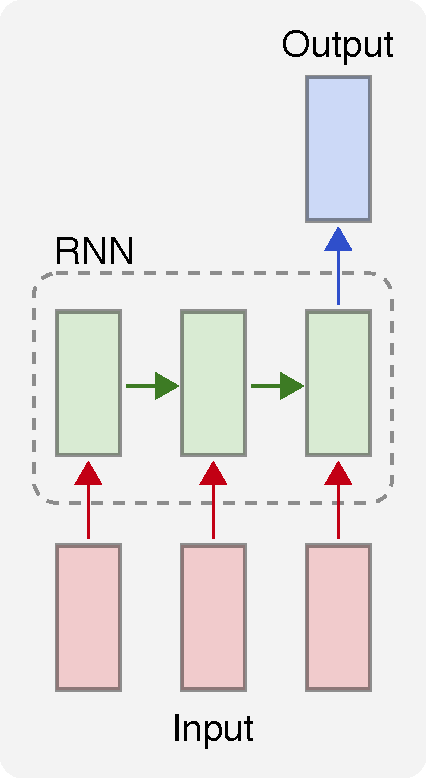
\includegraphics[width=0.24\textwidth]{figures/rnn}
    \caption{RNN Architecture known as Many-to-One \label{fig:rnn}}
    \vspace{-6pt}
\end{wrapfigure}

Different approaches have been proposed for both temporal and non-temporal sequences.
The state-of-the-art architecture for classifying temporal sequences is called Recurrent Neural
Network (RNN). Unlike classic feedforward neural networks, RNNs can use their internal memory 
to process arbitrary sequences of inputs. Their internal memory also allows them to remember
features vectors received at previous time instants which make them suitable for temporal
sequences. 

\st{* Why we chose Recurrent Neural Network, why the LSTM.}

One of the main problems with RNNs is the so-called vanishing gradient problem. In particular,
during the training phase, the gradient that is back-propagated from the last RNN (right-most 
RNN in Fig.~\ref{fig:rnn}) towards the first RNN (left-most RNN in Fig.~\ref{fig:rnn}) becomes
really small (vanishes) before reaching the head of the chain. This problem prevents the first
part of the network from learning. The longer is the chain, the more the network suffer
the vanishing gradient). Since in our case we work with long sequences of IMU readings, we used
the LSTM-RNN (Long Short-Term Memory RNN) which is specifically designed to avoid the 
vanishing gradient problem.

\st{* Let's introduce the fact that we do some data post-processing before feeding it to the model
(the next section will be about data post-processing).}

In order to make the dataset suitable for a machine learning approach, we need to apply
a post processing step (see ~\ref{subs:postproc} for details).

\newpage
\subsection{Data post-processing}\label{subs:postproc}
\vspace{-.3cm}
\textbf{Assigned to: Andrea}

\st{* Here we talk about the fact that we downsample the readings from $128Hz$ to $16Hz$. Let's
justify it by saying that we tried different factors and empirically chose the one that maximizes
reduction while preserving signal shape (we tried $2, 4, 8, 16, 32$).}

Since we feed the temporal sequence of readings from the accelerometer to the chain of RNNs,
we need as many RNNs as the number of readings in a single input. Our inputs are traces of
$10$ seconds each, with the IMU producing data at $\sim 128Hz$. Using the whole trace would
require a chain of $1280$ RNNs which is computationally prohibitive. 
\textbf{Observation 1:} In our
case, the fingerprints of all the activities that we are trying to classify present a periodic behavior.
This means that we don't need to focus on the entire trace but we can look at part of it. 
\textbf{Observation 2:} It is possible to down-sample our readings from $128Hz$ to a lower
rate as long as we don't loose the profile of the signals.

We empirically found that it is possible to classify one trace just by looking at $1$ seconds of
readings down-sampled by a factor of $8$. Thus, our chain of RNNs contains only $16$ cells.
We partition each trace from the training set into $10$ smaller samples of $1$ second each, 
and we treat them as independent samples.


\st{* Let's also talk about the trimming phase, in which we discard the first and last $2$ seconds
of each trace because of the time spent to say ''Now you can start jumping``, or the time
required to switch windows (while Driving the car) and the time when somebody stops earlier and
asks ''Can I stop jumping?``.}

Another observation is that, while collecting data, people tend to waste time right after started
logging and sometimes before the end of the log (e.g., time spent to switch window and start
driving the car, somebody stopped jumping too early). Using these bad samples to train the model
is not just useless (because they are not informative) but can also confuse the neural network (
i.e., by teaching it that zero acceleration means driving). For this reason, we ignore the first and 
last $2$ seconds in each trace.

We augment the feature vector by computing the first and second derivative (respectively, 
the Jerk, and the Jounce) of the acceleration along the three axis. This idea is driven by the
observation that the rate at which the acceleration changes over time is more informative
than the acceleration itself in activity recognition. We empirically found out that passing
the time instant as an extra feature along with the accelerometer data improves the performances
of the model.


\subsection{Recurrent Neural Network}
\vspace{-.3cm}
\textbf{Assigned to: Andrea}

\st{* Here we explain and show the architecture of our neural network by unwrapping the timesteps.}

\begin{figure}[t]
    \centering
    \vspace{-8pt}
    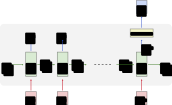
\includegraphics[width=0.8\textwidth]{figures/rnn_full}
    \caption{RNN Architecture known as Many-to-One \label{fig:rnn_architecture}}
    \vspace{-6pt}
\end{figure}



\st{* Explain what is X, what is Y, and what is the hidden state. Do not talk about batching here.}

Figure~\ref{fig:rnn_architecture} shows the architecture of the model that we used, where
$T \in [0,15]$ (i.e., $1$ second per sample at $16Hz$), $S_t$ is called hidden state of the
RNN at time $t$ and it represents the information passed by the RNN at time $t-1$ to the RNN
at time $t$ (with $S_0$ set to $0$ and $S_T$ discarded), $Z_t$ is called output of the RNN
at time $t$, $X_t$ is the vector of features at time $t$ and contains $10$ features, 
$Y \in [0,1,2,3]$ the output label indicating the activity that generated $X$. 
The $SoftMax$ block converts 
unnormalized logits returned by the last RNN into a probability distribution over classes.


\st{* Explain (briefly) the training process and how gradient back-propagation works.}

We train our model using Adam~\cite{kingma2014adam} for
optimization. The learning process is driven by the minimization of the cross-entropy loss
function~\cite{rubinstein1999cross}.

\subsection{Dataset}
\vspace{-.3cm} 
\textbf{Assigned to: Andrea}

\step{* Here we just talk about how much data (samples) we used for training, how much for
validation and how much for testing.}

We trained our model on $900$ samples of $16$ IMU readings each. We removed $144$ samples
from the training data and used it for testing our model and decide when to stop training.


\section{Results}
\vspace{-.3cm}
\textbf{Assigned to: Noah}

* Here we discuss and show a plot of the training/validation loss/accuracy over time (over epochs).

* We show the confusion matrix computed either on the validation set (if not cross-validation) or
on the training set (if cross-validation).

* Let's not forget to talk about merging PDs to get to the most likely label for one trace.


\section{Conclusion}
\vspace{-.3cm}
\textbf{Assigned to: Noah}

* Here we can talk about the possibility to deploy our model on mobile devices. Let's just say that 
there exist an implementation for mobile devices of tensorflow so our approach can be easily and 
seamlessly deployed on a mobile device.

\end{document}
